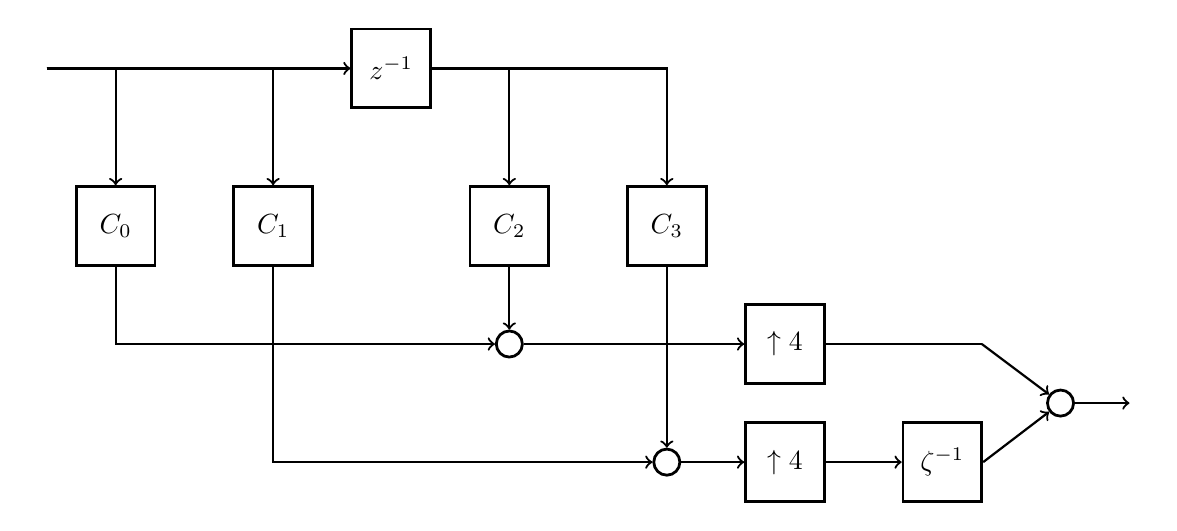
\begin{tikzpicture}
[	
	sq/.style={rectangle,draw,line width=1,minimum height=1cm,minimum width=1cm},
	rd/.style={circle,draw,line width=1,radius=0.5cm}
]

\node[sq] (t1) at (3.5,0) {$z^{-1}$};

\node[sq] (c1) at (0,-2) {$C_0$};
\node[sq] (c2) at (2,-2) {$C_1$};
\node[sq] (c3) at (5,-2) {$C_2$};
\node[sq] (c4) at (7,-2) {$C_3$};

\node (start) at (-1,0) {};

\draw[thick,->] (start) -| (c1);
\draw[thick,->] (start) -| (c2);
\draw[thick,->] (start) -- (t1);
\draw[thick,->] (t1) -| (c3);
\draw[thick,->] (t1) -| (c4);

\node[rd] (s1) at (5,-3.5) {};
\node[rd] (s2) at (7,-5) {};

\draw[thick,->] (c1) |- (s1);
\draw[thick,->] (c3) -- (s1);
\draw[thick,->] (c2) |- (s2);
\draw[thick,->] (c4) -- (s2);

\node[sq] (us1) at (8.5,-3.5) {$\uparrow 4$};
\node[sq] (us2) at (8.5,-5) {$\uparrow 4$};

\draw[thick,->] (s1) -- (us1);
\draw[thick,->] (s2) -- (us2);

\node[sq] (t2) at (10.5,-5) {$\zeta^{-1}$};
\draw[thick,->] (us2) -- (t2);

\node[rd] (s3) at (12,-4.25) {};
\node (p1) at (11,-3.5) {};

\draw[thick] (us1) -- (p1.center);
\draw[thick,->] (p1.center) -- (s3);
\draw[thick,->] (t2.east) -- (s3);

\node (end) at (13,-4.25) {};
\draw[thick,->] (s3) -- (end);

\end{tikzpicture}